	
	
	\section{Extended Moduli Spaces of Connections}
	Let $G$ be a unitary Lie group and let $\Sigma$ be a compact connected genus $g$ Riemann surface. Recall (Section \ref{s:moduli-as-reps}) that the moduli space of flat connections $\MM$ can be constructed as representations $\Hom(\pi_1(\Sigma),G)/G$, which has its subset topology as $\xi^{-1}(e)/G \subset G^{2g}/G$, where 
	\begin{equation}
		\xi(A_1,B_1,...,A_g,B_g) = \prod_{i=1}^g A_iB_iA_i^{-1}B_i^{-1}.
	\end{equation} 
	Now let us generalize to the case where $\Sigma$ is permitted to have $n$ punctures, $\{p_i\}_{i=1}^n$. Fix a point $p$ in a neighbourhood of $p_1$, and let $c_1$ be a loop around $p_1$ based at $p$. For each $i\neq 1$, let $c_i$ be a loop around $p_i$ in $\Sigma$, based at a point $q_i$ in a neighbourhood of $p_i$, and let $\{d_i\}_{i=2}^n$ be curves $d_i:p\to q_i$ in $\Sigma$. The path $k_j=d_jc_jd_j^{-1}$ is a loop based at $p$, and thus the fundamental group of $\Sigma$ can be written \cite[Eqn. 2.2]{hurtubise_representations_2000}:
	\begin{equation}
		\pi_1(\Sigma) = \left\langle a_i, b_i, c_1, k_j ~\bigg|~ \prod_{i=1}^{g}(a_ib_ia_i^{-1}b_i^{-1})c_1\prod_{j=2}^{n}k_j=e\right\rangle.
	\end{equation}
	Thus, we will redefine $\xi:G^{2g+2n-1}\to G$ to be
	\begin{equation}
		\xi(a_1,b_1,...,a_g,b_g,c_1,...,c_n,d_2,...,d_n) = \prod_{i=1}^{g}(a_ib_ia_i^{-1}b_i^{-1})c_1\prod_{j=2}^{n}d_jc_jd_j^{-1},
	\end{equation}
	and consider the set $\Hom(\pi_1(\Sigma),G)/G$, equipped with the subset topology $\xi^{-1}(e)/G\subset G^{2(g+n)-1}/G$.
	
	Suppose $\{C_i\}_{i=1}^{2g-g}$ is a trinion decomposition for an unpunctured surface $\tilde{\Sigma}$. Then, if we collapse a curve $C_j$ down to a single point $p_j$, we obtain a new surface $\Sigma$ with one puncture, which we desingularize into two punctures. From Proposition \ref{t:atd-thm}, any element $A$ in $\MM$ can be represented by an adapted to trinion decomposition (a.t.d.) connection (Def. \ref{d:atd-conn}), meaning that $A$'s holonomy around the curve $c_i$ corresponding to the point $p_i$ is in the maximal torus $\mathfrak{t}$. As a representation, this means we can choose a conjugacy class of $A$ with holonomy around $c_i$ in the fundamental alcove $\Delta \subset \mathfrak{t}$. If we repeat this for some $n$ curves in the trinion decomposition, the moduli space $\MM$ becomes the \emph{$T$-extended} moduli space
	\begin{equation}
		\MM^T := \{\left[(A_i,B_i)_{i=1}^{g},C_1,(D_j,C_j)_{j=2}^n\right]\in G^{2g+n-1}\times \exp(\Delta)^n ~|~ \xi(A_i,B_i,D_j,C_j) = \mathds{1}\}.
	\end{equation}
	We can also define the \emph{$G$-extended} moduli space:
	\begin{equation}
	\MM^G := \{\left[(A_i,B_i)_{i=1}^{g},C_1,(D_j,C_j)_{j=2^n}\right]\in G^{2g+n-1}\times G^n ~|~ \xi(A_i,B_i,D_j,C_j) = \mathds{1}\},
	\end{equation}
	and the map $\exp:\Delta\to\exp(\Delta)$ induces an inclusion $\MM^T \subset \MM^G$.
	\begin{theorem}
		The space $\MM^G$ is a smooth manifold, isomorphic to $G^{2(g+n-1)}$.
	\end{theorem}
	\begin{proof}
		The relation $\xi = 1$ allows us to write $C_1$ as a function of the other variables, which exhibits $\MM^G$ as the graph of a smooth function $G^{2(g+n-1)}\to G$.
	\end{proof}
	
	The conjugation action of $G$ gives an action on $\MM^G$, where an element $\sigma \in G$ acts by
	\begin{align*}
		A_j &\to \sigma A_j \sigma^{-1},& 	B_j&\to \sigma B_j\sigma^{-1}
	\end{align*}
	\begin{align*}
		D_j&\to \sigma D_j, & C_1 &\to \sigma C_1\sigma^{-1}
	\end{align*}
	For the punctures $l=2,...,n$, there is also an action of $G$ corresponding to changing the trivialization of the underlying bundle near the punctures. An element $\sigma$ in the $l$th copy $(l=2,...,n)$ of $G$ acts by
	\begin{align}
	\label{e:impl-action}
	D_l&\to D_l\sigma^{-1}, & C_l &\to \sigma C_l\sigma^{-1}.
	\end{align}
	This action of $G^n$ on $\MM^G$ restricts to give an action on $\MM^T$. Next we would hope to give $\MM^G$ some symplectic structure. It turns out, the appropriate structure is that of a \textit{quasi-Hamiltonian} $G$ \textit{space}. It is known that $\MM^G$ has a 2-form $\omega$ invariant under the $G^k$ action, and an equivariant \textit{moment map} $\Phi:\MM^G\to G$, given by $(A_i,B_i,D_j,C_j)\to C_k^{-1}$ \cite{alekseev_lie_1998}. 
	
	\section{Imploded Cross-Sections} 
	To proceed, we will state some definitions and results about \emph{imploded cross sections}, from e.g.\cite{alekseev_lie_1998} and \cite{jeffrey_imploded_2020}. The imploded cross-section is meant to take a quasi-Hamiltonian $G\times G$ space and reduce it to a quasi-Hamiltonian $G\times T$ space in two steps, similarly to a symplectic reduction. First, one restricts via the moment map to the fundamental alcove in $\mathfrak{t}$, and then one reduces the right $G$-action to a $T$-action by quotienting out the stabilizers of the maximal alcove in $\mathfrak{t}$.
	\begin{definition}
		For a quasi-Hamiltonian $G\times G$-space $M$ with moment map $\Phi$, and fundamental alcove $\Delta\subset \mathfrak{g}$, we define the imploded cross section 
		\begin{equation}
			M_{impl} := \prod_{\sigma} \frac{\Phi^{-1}(\sigma)}{[G_\sigma, G_\sigma]},
		\end{equation}
		where $\sigma$ ranges over the faces of $\Delta$, and $G_\sigma$ is the stabilizer of $\sigma$ under the action of $G$ by conjugation at a point in the interior of $\sigma$.
	\end{definition}
	\underline{Example}: Consider the double $D(G):=G\times G$, which is a quasi-Hamiltonian $G\times G$ space with the action
	\begin{equation}
		(g_1,g_2)\cdot (a,b) = (g_1 a g_2^{-1}, g_2bg_1^{-1}),
	\end{equation}
	and moment-map $\Phi:D(G)\to G\times G$ given by $\Phi(a,b)\to(ab,a^{-1}b^{-1})$. Let us introduce new co-ordinates $u=a$ and $v=ba$ for $D(G)$, in which the action becomes
	\begin{equation}
		(g_1,g_2)\cdot(u,v) = (g_1ug_2^{-1}, \Ad_{g_2} v),
	\end{equation}
	and the moment map becomes
	\begin{equation}
		\Phi(u,v) = (\Ad_u v, v^{-1}).
	\end{equation}
	For $G=SU(2)$, $T=S^1$, the implosion $D(G)_{impl}$ is smooth, isomorphic to $S^4$, and is a quasi-Hamiltonian $G\times T$-space. We only give a sketch here, the details can be found in \cite[Prop 2.29]{hurtubise_representations_2000}. For $SU(2)$, the fundamental alcove is $\Delta = [0,1]$, which has three faces, $\sigma_0 = (0,1)$, and $\sigma_{\pm} = \pm1$. For $\sigma_0$, we have $G_{\sigma_0} = T$ and hence $[G_{\sigma_0}, G_{\sigma_0}]$ is trivial. For $\sigma_\pm$, $G_\sigma = G = [G_\sigma,G_\sigma]$. For each face $\sigma$ of $\Delta$, the imploded cross-section has a stratum that is a quasi-Hamiltonian $G\times T$-space \cite[Theorem 5.1]{alekseev_lie_1998}.
		
	For the interior $\sigma_0$, we have $\Phi^{-1}(\sigma_0) = \{(u,v)\in D(G)~|~ v^{-1}\in \sigma^0\} = G \times \sigma^0$, hence $\Phi^{-1}(\sigma_0)/[G_{\sigma_0},G_{\sigma_0}] = G\times \sigma^0$. For the other faces $\sigma_{\pm}$, $\Phi^{-1}(\sigma_\pm) = \{(u,v)\in D(G)~|~ v^{-1} = \pm 1\} = G$, hence $\Phi^{-1}(\sigma_\pm)/[G_{\sigma_\pm},G_{\sigma_\pm}] = G/G = 1$. Therefore the imploded cross section is
	\begin{equation}
			D(G)_{impl} = (G\times \sigma^0) \coprod {1} \coprod {1}.
		\end{equation}
	One can identify this with $S^4$ by projecting the cylinder $(G\times \sigma^0) \cong S^3\times (-1,1)$ to $S^4$ without the north and south poles, and then identifying the two points with the poles. 
		
	The interior stratum $(G\times \sigma^0)$'s quasi-Hamiltonian structure is inherited from that of $D(G)$, and one must check explicitly that it extends to the other two points. The residual $G\times T$ action on $G\times \sigma^0$ is given by
	\begin{equation}
			(g,t)\cdot (u,v) = (gut^{-1},v),
	\end{equation}
	with moment maps $\Phi_G(u,v) = (uvu^{-1})$ and $\Phi_T(u,v) = v^{-1}$.

	To compute the imploded cross-section of our extended moduli spaces, we will use the following result, which tells us that $D(G)_{impl}$ is a \emph{universal} implosion \cite[Prop 2.32]{hurtubise_representations_2000}:
	\begin{theorem}
		Let $M$ be a quasi-Hamiltonian $H\times G$-space, where $G=SU(2)$, and let $D(G)_{impl}$ be the imploded cross-section of $D(G)$. Then
		\begin{equation}
			M_{impl} = M\times D(G)_{impl}\sslash G = {(m,\xi)\in M\times D(G)_{impl}~|~\Phi(m)=\Phi_G(\xi)}/G.
		\end{equation}
		The space $M_{impl}$ is a quasi-Hamiltonian $H\times T$ space, and it is smooth over the locus of points $(m,\xi)\in M\times D(G)_{impl}$ where the stabiliser of the $G$-action is trivial.
	\end{theorem}
	Next we will construct the symplectic implosion of the space $\MM^G$ which is a quasi-Hamiltonian $G^n$-space. There is an action of $G$ associated to each curve in our trinion decomposition for $\Sigma$, with moment map $\Phi_j$ given by just $C_j^{-1}$. Performing the implosion once for each puncture, the resulting space $\MM^G_{impl}$ will be denoted $P$, and it is a Hamiltonian $T^n$ space.
	
	After imploding the first $n-1$ punctures $(j=2,...,n)$, we obtain the set
	\begin{equation}
		\left\{
		(A_i,B_i,C_1,W_2,...,W_n)~|~ A_k,B_k,C_1 \in G, W_j \in D(G)_{impl},~ \prod_{j=1}^{g}[A_j,B_j]C_1\prod_{j=2}^{n} \Phi_G(W_j) = 1 
		\right\}.
	\end{equation}
	In terms of the $(u,v)$ co-ordinate for $D(G)$, $W_j = (u,v)$ with $u=D_j$ and $v = C_j$. To finish the imploded cross-section, it remains to implode the cross-section for the action of the first copy of $G$ appropriately. Let $W_1 = (\mathds{1},C_1)$ in $G\times G$ and define an action of $G$ by
	\begin{equation}
		\label{e:first-action}
		\left(A_k,B_k,W_j=(u_j,v_j)\right) \to (gA_kg^{-1}, gB_kg^{-1}, (gu_j,v_j)).
	\end{equation}
	Then the final imploded cross-section $P$ becomes \cite{hurtubise_representations_2000}
	\begin{equation}
		\label{e:P-def}
		P = \left\{(A_k,B_k,W_1,...,W_n)~|~ \coprod_{j=1}^g[A_j,B_j]\coprod_{j=1}^n \Phi_G(W_j)=1\right\}.
	\end{equation}
	There is a natural map from $\MM$ to $P$:
	\begin{lemma}
		There is a surjective map $\phi:\MM\to P$ which is a bijection over the interior $(\Delta^0)^n$ of the moment polytope. 
	\end{lemma}
	\begin{proof}
		For each puncture $p_k$, the corresponding imploded cross-section is given by the strata
		\begin{equation}
			\Phi_k^{-1}(\sigma)/[G_\sigma, G_\sigma]
		\end{equation}
		for each face $\sigma \in \Delta$ in the fundamental chamber of the $k$-th copy of $G$. The inverse image $\Phi_k^{-1}(\Delta)$ are those elements with $C_k^{-1} \in T$, and therefore the elements in $\bigcap_k \Phi_k^{-1} (\Delta)$ is exactly $\MM$. Then the quotient map on each strata defines a surjection $\phi:\MM\to P$. Over the interior $\Delta^0$ of each implosion, the quotient is trivial so $\phi$ is the identity map, which is bijective. 
	\end{proof}
	\begin{theorem}
		Over $(\Delta^0)^n$, $\phi:\MM \to P$ is a symplectomorphism.
	\end{theorem}
	\begin{proof}
		Hurtubise and Jeffrey \cite[Proposition 2.37]{hurtubise_representations_2000}.
	\end{proof}
	

	\pagebreak
	Now associated to the compact Riemann surface $\Sigma$ we have a symplectic variety $P$ of representations with weighted frames, which is toric for $G=SU(2)$ and has a prequantum line bundle $\LL_P$ corresponding to $\LL$ on $\MM$. Now we will go in detail on the other half of Jeffrey and Hurtubise's construction, building the complex variety $\cP$ of \emph{framed parabolic bundles} over a singular curve $\tilde{\Sigma}$ corresponding to contracting the loops in a trinion decomposition of $\Sigma$. We will see that $P$ and $\cP$ are diffeomorphic, meaning that we can compute sections of prequantum line bundles over $\cP$ using the structure of $P$.
	
	First we see how to embed $\MM$ into projective space using determinants, as this construction will have us transform the data of $\MM$ from holomorphic bundles over $\Sigma$ to sheaves, which is the perspective we will use to construct $\cP$.
	\section{Projective Embedding of $\MM$}
	\label{s:m-embedding}
	The moduli $\MM$ of flat $SL(n,\C)$ bundles can be embedded into projective space using the sections of the determinant bundle over $\MM$. There is a construction of this embedding due to Bhosle \cite{bhosle_parabolic_1989}, which we describe following Thaddeus and Gieseker \cite[\S 7]{thaddeus_geometric_1996}\cite{gieseker_moduli_1977}. 
	
	First, fix a line bundle $L$ of sufficiently high degree so that for all $E\in N(k,d)$, $E\otimes L$  is globally generated, and redefine $E$ as $E\otimes L$. Then, for some large $N$ we can write $E$ as a quotient:
	\begin{equation}
	\phi:\OO^N \to E.
	\end{equation}
	This quotient induces a map from $\wedge^k(\OO^N) \to \wedge^k(E)$ and the $SL(k,\C)$ structure induces an isomorphism $\mu:\wedge^k(E)\cong L^k$. Hence, a quotient of the trivial bundle induces an element $\hat{\beta}$ in 
	\begin{equation}
	V_1 := \Hom(H^0(\wedge^k(\OO^N)), H^0(L^2)).
	\end{equation}
	Now to pass to $\MM$ we quotient by $GL(k,\C)$. Suppose we have $\phi_2 = \Lambda^{-1} \phi_1 \Lambda$. Then
	\begin{equation}
		\hat{\beta}_2 = \mu(\wedge^k \phi_2) = \mu(\wedge^k \Lambda^{-1}\phi_1 \Lambda) = \det\Lambda \mu(\wedge^k \phi_1) = \det\Lambda~ \hat{\beta}_1.
	\end{equation}
	Therefore the orbits of $GL(k,\C)$ correspond to equivalence classes in $\PP(V_1)$. It is this mapping, which we will denote $\iota:\MM\to \PP(V_1)$, which we claim is an embedding. 
	\begin{lemma}
		The map $\iota:\MM \to \PP(V_1)$ is injective.
	\end{lemma}
	\begin{proof}
		 Suppose $(E_1, \dbar_{E_1})$ and $(E_2, \dbar_{E_2})$ are holomorphic vector bundles for which $\hat{\beta}_1 = \iota(E_1) = \iota(E_2) = \hat{\beta_2}$. Since the $SL(k,\C)$ structure is unique up to $\C^\ast$, this means that
		\begin{equation}
		\wedge^k \phi_1 = \lambda \wedge^k \phi_2
		\end{equation}
		for some $\lambda \in \C^\ast$. Fixing a local trivialization of $E_1$, $E_1|_U \cong U\times \C^k$, and picking a local frame $e_1,..,e_k$, choose any sections $s_1,...,s_k \in \OO^N|_{U}$ so that $\phi_1(e_i) = s_i$. Let $s = s_1 \wedge s_2 \wedge ... \wedge s_k$. Then
		\begin{equation}
		e_1\wedge...\wedge s_k=\phi_1(s_1)\wedge...\wedge \phi_1(s_k)= \wedge^k \phi_1(s) = \lambda \wedge^k \phi_2(s) = \lambda \phi_2(s_1)\wedge...\wedge \phi_2(s_k)
		\end{equation}
		Since $\{e_i\}$ was a local frame, the left-hand-side is non-zero, and the right-hand-side is also non-zero. Therefore $\{\phi_2(s_i)\}$ is a local frame trivializing $E_2$ on $U$. This map $e_i \to \phi_2(s_2)$ gives an isomorphism of $E_1$ with $E_2$. Note that this isomorphism is not unique as we could have picked other sections $\tilde{s}_i$ with $\phi_1(\tilde{s}_i) = e_i$.
	\end{proof}
	\begin{theorem}
		\label{t:det-embed}
		The map $\iota:\MM \to \PP(V_1)$ is an embedding.
	\end{theorem}
	\begin{proof}
		From the lemma, we know $\iota$ is injective, and thus it remains to show that $d\iota$ is injective. We give a proof following Thaddeus \cite[Prop 7.1]{thaddeus_geometric_1996}.
		
		Recall that the tangent space $T_\phi \MM = H^1(\End E)$ (Section \ref{s:ss-bundles}), for $\phi:\OO^N \to E$. Before quotienting $GL(k,\C)$, the map $\iota$ was given by the sending $\phi \to \hat{\beta} \in V_1$ which is essentially $\phi \to \wedge^k \phi$. Thus, we expect the derivative $T_\phi\MM\to V_1$ to be essentially $\psi \to \wedge^{k-1}\phi \wedge \psi$, for $\psi \in T_\phi \MM$. Precisely, if we deform the quotient map $\phi$ to $\phi + \epsilon\psi$ with $\epsilon^2 = 0$, then we have
		\begin{equation}
			\wedge^k (\phi+ \epsilon\psi) = \wedge^k(\phi) + \epsilon\wedge^{k-1}\phi\wedge \psi.
		\end{equation}
		Then taking the $GL(k,\C)$ quotient gives the map $d\iota$. Hence to show $d\iota$ is injective, we want to show that $\wedge^{k-1}\phi \wedge \psi =0$ only if $\phi+\epsilon \psi = \phi \mod GL(k,\C)$. To show this, we use the following linear algebraic lemma \cite[Lemma 7.2]{thaddeus_geometric_1996}
		\begin{lemma}
			If $\phi:\C^n \to \C^k$ is a linear surjection and $\psi:\C^n\to\C^k$ is a linear map, then $\wedge^{k-1}\phi\wedge\psi =0$ if and only if $\psi = f\phi$ for some $f\in \End \C^k$ with trace zero.
		\end{lemma}
		This lemma tells us that if $\wedge^{k-1}\phi\wedge\psi=0$ then $\psi = f\phi$ and hence $\phi+\epsilon\psi = \phi(1 + \epsilon f)$. Then since $f$ is traceless, $1+\epsilon f$ is in $GL(k,\C)$, so $d\iota$ is injective.
	\end{proof}

	\section{Parabolic Vector Bundles}
	Given a trinion decomposition of the Riemann surface $\Sigma$, let us fix the holonomies around each boundary loop. If we think of each trinion as a thrice-punctured sphere and consider the space of connections with fixed holonomies on the trinion, then due to Mehta and Seshadri (cite) there is a correspondence between the moduli of $\pi_1(\Sigma)$ representations into $SU(n)$ and that of rank-$n$ holomorphic bundles with an $SL(n,\C)$ structure and a parabolic structure at the punctures of $\Sigma$, which we call a parabolic bundle. Under this correspondence, the eigenvalues of the holonomy get translated into a set of weights for the parabolic structure. 
	
	We want to consider the moduli space of connections with all possible holonomies, and therefore we will want to fit all these moduli of parabolic bundles together, and in such a way that we can even include the $\theta_i = 0,\pi$ cases, which will correspond to weights $0$ and $1$. This is the construction of Hurtubise and Jeffrey which we will describe in the next section. First we lay out the basic definitions and results about parabolic bundles.
	\begin{definition}
		A \emph{parabolic bundle} over a complex manifold $\Sigma$ is a holomorphic vector bundle $E$ over $\Sigma$ with a \emph{parabolic structure}, which is a point of marked points $\{p_1,...,p_n\}$ and for each point, a flag of subspaces in the fibre $E_{p_k}$. 
	\end{definition}
	In particular if $E$ has rank 2, then a parabolic structure on $E$ is a choice of points $\{p_k\}$ and a sheaf homomorphism $\alpha:E\to S$ where $S := \bigoplus_{k} \C_{p_k}$.
	
	There is an adapted notion of stability for parabolic vector bundles.
	\begin{definition}
		\label{d:para-stable}
		Let $\gamma_1,...,\gamma_n \in [0,1]$ be a set of weights. For a subbundle (not necessarily proper) $F$ of $E$ we set $\mu_i(F) = 1$ if $F_{p_i} \subset \ker\alpha_i$, and $\mu_i = 0$ otherwise. Define $\sigma(F) = \frac{1}{rk(E)}$ if $F=E$ and $0$ otherwise. Then we say a pair $(E,\alpha)$ is \emph{stable} with respect to $\gamma$ if 
		\begin{equation}
		rk(E)\deg(F) < rk(F)\left(\deg(E) - \sum_{i=1}^n \gamma_i\right) 
		+ rk(E)\sum_{i=1}^n(1 - \mu_i(F) + \sigma_i(F))\gamma_i.
		\end{equation}
		If the inequality is not strict, $(E,\alpha)$ is \emph{semi-stable}.
	\end{definition}
	 Let us summarize some important results about weighted parabolic bundles.
	\begin{lemma}
		\label{l:ss-lemma}
		If $(E,\alpha)$ is a parabolic bundle semi-stable with respect to weights $\gamma$, then:
		\begin{enumerate}
			\item The kernel of $\alpha$ is torsion free, and the torsion subsheaf of $E$ is non-zero only at the $p_i$, equalling $0$ or $\C$ at each $p_i$.
			\item If $\gamma_i >0$, then $\alpha_i \neq 0$.
			\item If $\gamma_i < 1$, then $E$ is torsion free at $p_i$.
			\item If $\gamma_i \in (0,1)$, one has a parabolic structure at $p_i$, and if all the weights are in $(0,1)$, then $(E,\alpha)$ is stable with respect to $\gamma$, if and only if it is stable with respect to weights $(1-\gamma_i)/2$ and $(1+\gamma_i)/2$.
			\item If $(E,\alpha)$ is locally free at $p_i$ and $\alpha \neq 0$, then for $\gamma_i = 0$, there is a family $(E_t, \alpha_t)$, $t\in \C$, of semi-stable pairs such that $(E_t,\alpha_t)\cong (E,\alpha)$ for $t\neq 0$, and $\alpha_0 = 0$. 
			\item If $(E,\alpha)$ is locally free at $p_i$ and $\alpha \neq 0$, then for $\gamma_i = 1$, there is a family $(E_t,\alpha_t)$, $t\in \C$, such that $(E_t, \alpha_t)\cong (E,\alpha)$, $t\neq 0$ and $E_0$ has torsion at $p_i$.
		\end{enumerate}
	\end{lemma}
	\begin{proof}
		Hurtubise and Jeffrey \cite[Lemma 4.3]{hurtubise_representations_2000}
	\end{proof}
	One consequence of this lemma is that when $\gamma_i\in (0,1)$, the set of semi-stable parabolic bundles is torsion-free. The weights $\gamma_i$ will correspond to holonomy angles of flat $SU(2)$ connections around curves in a trinion decomposition, and so weights in $(0,1)$ correspond to non-central holonomies. There are two edge cases to consider: when $\gamma_i = 0$, the parabolic structure vanishes, and when $\gamma_i = 1$ we acquire torsion. To fit all connections with all possible holonomies into a moduli space, each of these cases will need to be dealt with.
	
	\section{Moduli of Framed Parabolic Bundles}
	Here we construct a moduli space of parabolic vector bundles. This section closely follows Hurtubise and Jeffrey \cite[\S 4]{hurtubise_representations_2000}. From now on, we restrict our attention to $G=SU(2)$. Let $\Sigma$ be a compact connected Riemann surface with $n$ punctures $\{p_i\}_{i=1}^n$. Fix a line bundle $L$ of sufficiently high degree so that for all $E\in N(k,d), E\otimes L$ is a globally generated sheaf (and redefine $E = E\otimes L$). Then for some large $N$ we can write $E$ as a quotient of the trivial sheaf on $\Sigma$:
	\begin{equation}
		\phi: \OO^N \to E.
	\end{equation}
	Just as in Section \ref{s:m-embedding} we have a mapping $\hat{\beta}$ taking $E$ to the vector space $V_1 := \Hom(H^0(\wedge^k(\OO^N)), H^0(L^2))$. Now we add the parabolic data. At a point $p_i$, the map $\alpha_i:E\to \C_{p_i}$ pulls back to $\hat{\alpha}_i = \alpha_i\circ \phi$ in $V_2 := H^0(\OO^N)^\ast$. Since we are only interested in $\alpha_i$ up to (independent) scaling, the parabolic bundle $(E,\alpha)$ represents an equivalence class in
	\begin{equation}
		Z := \PP(V_1) \times \PP(V_2) \times ... \times \PP(V_2),
	\end{equation}
	where there are $n$ copies of $\PP(V_2)$, one for each puncture. Then letting $\tilde{\MM}$ denote the set of parabolic vector bundles on $\Sigma$, and $\tilde{\iota}:\tilde{\MM}\to Z$ denote the map taking $(E,\alpha)$ to $(\hat{\beta},\hat{\alpha})$, we get a closed subvariety $X = \tilde{\iota}\left(\tilde{\MM}\right)$ in $Z$. 

	Now we also have weights $\gamma = (\gamma_1,...,\gamma_n)$ for the parabolic structure. These vary the choice of polarization of $X$, namely the choice of line bundles on which the action of $SL(N,\C)$ \textit{linearises}. Let us recall what this means:
	\begin{definition}
		Given a linear algebraic group $G$ and a $G$-variety $X$, a line bundle $p:L\to X$ \emph{linearises} if there is an action of $G$ on $L$ such that for all $l\in L$, $g\in G$,
		\begin{equation}
			p(g\cdot l) = g\cdot p(l),
		\end{equation}
		and which restricts to a linear isomorphism $L_x \cong L_{g\cdot x}$ on fibres.
	\end{definition}
	In this case $G\cong SL(N,\C)$ which acts on $V_1$ and each copy of $V_2$.
	
	
	Let $\pi_1:Z \to \PP(V_1)$ and $\pi_{2,i}:Z\to \PP(V_2)$ denote the projections to the first factor and to the i-th factor of $Z$ respectively. Let
	\begin{equation}
		L_0 = \pi_1^\ast(\OO(N)),~ \text{ and } ~ L_{1,i} = \pi_1^\ast(\OO(N-1))\otimes \pi_{2,i}^\ast (\OO(2)).
	\end{equation}
	Then the linearisation corresponding to weights $\gamma = (\gamma_1,...,\gamma_n)$ is 
	\begin{equation}
		L_\gamma = (L_0)^{s_0} \otimes \left(
		\otimes_{i=1}^n (L_{1,i})^{s_{1,i}}
		\right),
	\end{equation}
	where $s_0(\gamma_i) = s_{1,i}(1-\gamma_i)$.
	
	In summary, for each set of weights $\gamma$, we have a corresponding moduli space of parabolic bundles that are semi-stable with respect to those weights, with $\gamma_i \neq 0,1$. Next we will fit these spaces together, and in such a way that we can include $\gamma_i = 0,1$. To do this, we put a $(\PP^1)^n$-bundle over $X$,
	\begin{equation}
		Y = \PP(L_0\oplus L_{1,1})\oplus \PP(L_0\oplus L_{1,2})\oplus ... \oplus \PP(L_0\oplus L_{1,n}).
	\end{equation}
	We endow $Y$ with the natural polarisation $\OO(1,1,...,1)$. Now $Y$ contains all the stable points for the various choice of weights, which correspond to the various possible holonomies of the unitary connections. We still need to account for gauge equivalence, which suggests we take the $SL(N,\C)$ quotient. This is not quite correct, as one must make an adjustment to account for the possibility that $\gamma_i = 0,1$.
	
	Consider a weighted parabolic bundles as a quadruple $(E, \alpha_i, A_i, \gamma)$, where $\alpha_i:E\to \C_{p_i}$ is the parabolic structure, $A_i$ is a subspace of $E_{p_i}$, with $A_i = \ker\alpha_i$ whenever $\alpha_i \neq 0$ (equiv. $\gamma \neq 0$), and $\gamma$ are the weights as usual. For $\gamma_i \neq 0$, we have not added any new information and when $\gamma_i = 0$ we are adding a projective class $A_i$ for the parabolic structure even as the map vanishes. On the other hand when $\gamma_1 = 1$, the sheaves can acquire torsion. To handle this, we first need
	\begin{lemma}[H\& J Lemma 4.11]
		Let $E_t$, $t\in\C$ be a family of coherent rank 2 sheaves over $\Sigma$, with $E_t$ locally free at $p$ for $t\neq 0$, and with $E_0$ having torsion subsheaf $\C_p$ near $p$. Let $\phi_t \in H^0(\Sigma, \wedge^2(E)^\ast)$ be a family of $SL(2,\C)$ structures on $E_t$. Then $\phi_0$ vanishes at $p$.
		\label{t:sl2-lemma}
	\end{lemma}
	\begin{proof}
		If $z$ is a local co-ordinate on $\Sigma$ on an open set containing $p$, such that $z(p)=0$, one can obtain $E_t$ locally (up to reparameterization) from the exact sequence 
		\begin{equation}
			\OO \xrightarrow{(0,t^k,z)} \OO \oplus \OO \oplus \OO \xrightarrow{~~~~~}E_t
		\end{equation}
		for some integer $k$. Then the $SL(2,\C)$ structures $\phi_t$ are multiples of $e_1^\ast \wedge (-ze^\ast_2 + t^k e^\ast_3)$, which vanishes when $z=t=0$.
	\end{proof}
	Since $Y$ is a projective bundle, one can freely tensor with line bundles and write $Y$ as the bundle
	\begin{equation}
		Y = \bigoplus_{i=1}^n\PP\left(\pi_1^\ast\left(
		\OO(-1)
		\right)\oplus \pi_{2,i}^\ast\left(\OO(-2)\right)\right).
	\end{equation}
	In this form, when $\gamma \neq 1$ there is a natural lift of a parabolic bundle $(E,\alpha)\in X$ to $Y$, given by 
	\begin{equation}
		\hat{E} = \left(
		(\hat{\beta}, \hat{\alpha}_1^2),(\hat{\beta},\hat{\alpha}_2^2),...,(\hat{\beta},\hat{\alpha}^2)
		\right),
	\end{equation}
	which we want to extend to the torsion case where $\gamma = 1$. When there is torsion at say $p_i$ ($\gamma_i = 1)$, one can rescale the torsion subsheaf of $E$, modifying $\hat{\alpha}_i^2$ to $c\hat{\alpha}_i^2$ for some $c$. This rescaling should remain in the same equivalence class, and if $\hat{\beta} \neq 0$ then since $\hat{\beta}$ is not rescaled this would not be the case. Therefore we want that the $i$-th component of the lift of $E$ in $Y$ should be $(0,\hat{\alpha}_i^2)$. This is achieved as follows; recall that $\hat{\beta}$ is defined by composing
	\begin{equation}
		\wedge^2(\OO^N) \xrightarrow{\phi} H^0(\Sigma, \wedge^2 E) \xrightarrow{\xi} H^0(\Sigma, L^2)
	\end{equation}
	where $\phi:\OO^N \to E$ is a quotient defining $E$. Recall that $E$ was defined as $E_0\times \LL$ for some bundle $E_0$ with $SL(2,\C)$ structure defining a map $\xi:H^0(\Sigma, \wedge^2(E_0))\to H^0(\Sigma,\OO)$. Therefore, we have a commutative diagram:
	\begin{equation}
		\begin{tikzcd}
			{H^0(\Sigma, \wedge^2(E_0))} && {H^0(\Sigma,\OO)} \\
			\\
			{\wedge^2(E_0)|_{p_i}} && \C
			\arrow["{\xi}", from=1-1, to=1-3]
			\arrow["{ev_{\OO}}", from=1-3, to=3-3]
			\arrow["{\xi^{p_i}}", from=3-3, to=3-1]
			\arrow["{ev_{\wedge^2(E_0)}}", tail reversed, no head, from=3-1, to=1-1]
		\end{tikzcd}
	\end{equation}
	Thus one has $\xi = \text{ev}_\OO^{-1}\circ \xi^{p_i} \circ \text{ev}_{\wedge^2(E)}$, and so for $\gamma_i=1$ we use this definition to define $\xi^{p_i}$ at the torsion points of $E$. Then, from Lemma \ref{t:sl2-lemma}, one has that $\hat{\beta}_i$ vanishes when there is torsion at $p_i$. Using this definition we can define a lift for all $(E,\alpha)\in X$ to $Y$ by $
	\hat{E} = \left(
	(\hat{\beta}, \hat{\alpha}_1^2),(\hat{\beta},\hat{\alpha}_2^2),...,(\hat{\beta},\hat{\alpha}^2)
	\right).$
	
	Next Hurtubise and Jeffrey analyse which elements of $Y$ are stable or semistable as weighted parabolic bundles. In Lemma \ref{t:sl2-lemma} we saw that torsion in the kernel of $\alpha_i$ destabilised $(E,\alpha) \in X$. The same is true in $Y$:
	\begin{lemma}[Hurtubise and Jeffrey, Lemma 4.13]
		A semi-stable element $y\in Y$ corresponds to a parabolic bundle $(E,\alpha)$ with no torsion in the kernel of $\alpha$.
	\end{lemma}
	To allow the $\alpha_i$ to go to zero but still preserve the information of which projective class we have at $p_i$, we define a new map. Let $(E,\alpha)\in X$ with $SL(2,\C)$ structure $\phi$. Then we can map $(E,\alpha,\phi)\to Y$ by
	\begin{equation}
		(E,\alpha,\phi) \to \bigoplus_{i=1}^n\left(
		(\phi(p_i)^N, \phi(p_i)^{N-1}\alpha_i^2
		\right),
	\end{equation}
	and we define $\hat{Y}$ to be the closure in $Y$ of the image of this map. In this closure, one obtains the points with $\alpha_i =0$. Then since $\phi(p_i)\neq 0$, Lemma \ref{t:sl2-lemma} guarantees $E$ is torsion free at $p_i$. The next proposition addresses stability:
	\begin{theorem}[Hurtubise and Jeffrey, Prop. 4.14]
		Let 
		\begin{equation}
			y = \left(
			(b_1, a_1), (b_2, a_2),...,(b_n, a_n)
			\right)
		\end{equation}
		be a point in $\hat{Y}$. Let $\Gamma(y)$ be the set of $\gamma_i \in [0,1]$ such that $\gamma_i =0$ if $a_i =0$ and $\gamma_i = 1$ if $b_i = 0$. Then $y$ is semi-stable if and only if for one element $\gamma \in \Gamma(y)$, $\pi(y)\in X$ is $\gamma$-semi-stable.
	\end{theorem}
	Therefore semi-stable elements in $\hat{Y}$ all project down to semi-stable elements of $X$ for some choice of weights, and the GIT quotient $\hat{Y}\sslash SL(N,\C)$ corresponds to equivalence classes of quadruples $(E,\alpha_i, \hat{\alpha}_i, \phi)$ where $(E,\alpha)$ is a parabolic bundle, $\hat{\alpha}_i$ is a subspace of $E|_{p_i}$ (which is the kernal of $\alpha_i$ when $\alpha_i \neq 0$) and $\phi$ is an $SL(2,\C)$ structure. However this is not quite the final moduli space we want to construct, as we have added the extra information of $\hat{\alpha}_i$ when $\alpha_i = 0$. At these points, $\hat{\alpha}_i \in \PP_1=\PP(E|_{p_i})$. We want to collapse these extra $\PP_1$s. To do this, embed $V_1$ into $W_1 = V_1^{\otimes N}$ so that a non-zero element $l$ in $L_{0} = \pi_1^\ast(\OO(N))$ can be thought of as an element in $W_1^\ast$ by taking $v_1\otimes...\otimes v_n$ to $l(v_1)l(v_2)...l(v_n)$. Similarly, embedding $V_2$ into $W_2 = V_1^{\otimes N-1}\otimes V_2\otimes V_2$ allows us to think of non-zero elements in $L_{1,i}$ as elements of $W_2^\ast$. Then this maps $\hat{Y}$ to a subvariety $\tilde{Y}$ in $\prod_{i=1}^n \PP(W_1\otimes W_2)$, and the map collapses the unwanted $\PP_1$s while being an embedding otherwise. 
	
	Finally, we let $\cP = \tilde{Y}\sslash SL(N,\C)$ be the geometric quotient, and we call it the \emph{moduli space of framed parabolic bundles}.
	
	Remark: Here the quotient is meant to be taken in the sense of Geometric Invariant Theory; the resulting space consists of the stable and semi-stable orbits of the $SL(N,\C)$ action on $\tilde{Y}$, where stable means the orbit is closed and the stabiliser is finite, semi-stable means $0$ is not in the closure of the orbit, and unstable means $0$ is in the closure. These definitions agree with Definitions \ref{d:stable} and \ref{d:para-stable} for vector bundles and parabolic sheaves.
	
	
	\section{Framed Parabolic Bundles on a Trinion}
	To understand the moduli space of framed parabolic bundles on a (punctured) Riemann surface, one can mirror the construction of section 3 and decompose the punctured Riemann surface into trinions. Towards this end, let us compute $\cP$ for one trinion $D$, a copy of $\PP^1$ with three marked points. Up to a birational map, let the three marked points be $z=0,1,\infty$. 
	
	\begin{lemma}
		\label{t:four-seqs}
		A degree-0 framed parabolic sheaf $(E,\alpha)$ on $D$ which is semi-stable must fall into one of four cases:
		\begin{enumerate}
			\item $E$ is trivial; $E\cong \OO\oplus \OO$.
			\item $E$ is torsion-free but not trivial, and $E\cong \OO(1)\oplus\OO(-1)$.
			\item $E$ has torsion at one point $p$, and $E\cong \OO\oplus\OO(-1)\oplus \C_p$.
			\item $E$ has torsion at two points $p_1,p_2$, and $E\cong \OO(-1)\oplus\OO(-1)\oplus\C_{p_1}\oplus \C_{p_2}$.
		\end{enumerate}
	\end{lemma}
	\begin{proof}
		Suppose that $E$ has no torsion. Then $E \cong \OO(j)\oplus \OO(-j)$, $j\in\mathbb{Z}$. If $E$ is semi-stable with respect to some weights $\gamma$, the semi-stability condition is that for all subbundles $F$ of $E$,
		\begin{equation}
			2\deg(F) \leq rk(F)\left(
			0-\sum_{i=1}^n \gamma_i
			\right) + 2\sum_{i=1}^n(1-\mu_i(F) + \sigma(F))\gamma_i,
		\end{equation}
		where we recall that $\sigma(F) = \frac{1}{rk(E)}$ if $F=E$ and $0$ otherwise, and $\mu_i(F) = 1$ is $F_{p_i} \subset \ker \alpha_i$ and $0$ otherwise. Consider $F = \OO(j)$. The equation becomes
		\begin{equation}
			2j \leq \sum_{i=1}^n \gamma_i - 2\mu_i(F).
		\end{equation}
		Since $\gamma_i \leq 1$, This can never be satisfied for $j \geq 2$, and therefore $E = \OO\oplus\OO$ or $E=\OO(1)\oplus\OO(-1)$ are the only choices which can yield a semi-stable parabolic sheaf. 
		
		When $E$ has torsion at one of the marked points, say $p$, then let $E' = E/\text{Tor}(E)$.
		which is a bundle with $E\cong \OO(j-1)\oplus\OO(-j)$. Let $F=\OO(j-1)\oplus \C_p$. Then the stability condition for $E$ and $F$ is
		\begin{equation}
			2j \leq \sum_{i=1}^3 \gamma_i -2\mu_i(F)
		\end{equation}
		The right-hand side is at most 3, and therefore if $j\geq 2$ then the sheaf $\OO(j-1)\oplus \C_p$ is destabilising. Therefore we must have $E' \cong \OO(-1)\oplus \OO$, and $E \cong \OO(-1)\oplus \OO \oplus \C_p$. 
		
		If $E$ has two torsion points, then $E'\cong \OO(-j)\oplus\OO(j-2)$ If $j\geq 2$, then $\OO(j-2)\oplus \C_{p_1}\oplus \C_{p_2}$ will be destabilizing. If $j=0$, then $F=\OO\oplus\C_{p_1}\oplus \C_{p_2}$ has stability condition
		\begin{equation}
			4 \leq \sum_{i=1}^3 \gamma_i - 2\mu_i(F).
		\end{equation}
		The left hand side is at most 3, so $F$ is destabilizing. So $E' \cong \OO(-1)\oplus \OO(-1)$ is the only semistable choice, and $E \cong \OO(-1)\oplus \OO(-1)\oplus \C_{p_1} \oplus \C_{p_2}$. 
		
		Finally, if $E$ has torsion at all three marked points, $E' = \OO(-j)\oplus \OO(j-3)$. Then from Lemma \ref{l:ss-lemma}, $\gamma_i = 1$ for all $i$, $\mu_i = 0$ for all $i$.  Therefore the stability condition for the subsheaf $F=\OO(j-3)\oplus\C_{0}\oplus \C_{1}\oplus \C_{\infty}$ becomes
		\begin{equation}
			2j \leq -3 + 2(3) = 3
		\end{equation}
		This rules out $j\geq 2$. For $j=0,1$ the subsheaf $\OO(-j)\oplus\text{Tor}(E)$ will be destabilizing; the stability condition is
		\begin{equation}
			2(3-j) \leq 3.
		\end{equation}
		Hence there are no semi-stable sheaves $E$ with torsion at three points.
	\end{proof}
	\begin{theorem}
		\label{t:exactseq}
		For all degree-0 semi-stable parabolic sheaves $(E,\alpha)$ over $D$, $E\otimes \OO(1)$ is generated by four global sections. In particular, there is an exact sequence:
		\begin{equation}
		\OO(-2)\oplus \OO(-2) \xrightarrow{Az+Bz^{-1}} \OO(-1)^{\oplus 4} \xrightarrow{} E \to 0.
		\end{equation}
		With $A,B$ represented by $4\times 2$ matrices. The map $\OO(-2)\oplus \OO(-2) \xrightarrow{Az+Bz^{-1}} \OO(-1)^{\oplus 4}$ is injective as a map of bundles away from the torsion points of $E$.
	\end{theorem}
	\begin{proof}
		From the lemma, $E\otimes \OO(1)$ falls into one of four cases, each of which is a quotient of $\OO^{\oplus 4}$. In each case, the sequence defining $E\otimes \OO(1)$ can be written as a direct sum of the following exact sequences:
		\begin{enumerate}
			\item $\OO(-1) \hookrightarrow \OO^{\oplus 2}\twoheadrightarrow \OO(1) $
			\item $\OO(-1)^{\oplus 2} \hookrightarrow \OO^{\oplus 3} \twoheadrightarrow \OO(1)$
			\item $0 \hookrightarrow \OO \twoheadrightarrow \OO$
			\item $\OO(-1)\hookrightarrow \OO \twoheadrightarrow \C_p$.
		\end{enumerate}
		In any case, $E\otimes \OO(1)$ is generated by four global sections, and the kernel is $\OO(-1)\oplus \OO(-1)$. Thus tensoring with $\OO(-1)$ to recover $E$, we obtain the claimed exact sequence.
		
		Since $E$ is rank 2 away from torsion, and $E = \OO(-1)^{\oplus 4}/\text{im}(Az+Bz^{-1})$ by exactness, at every point $p$ without torsion $\text{im}(Az+Bz^{-1})|_p = \text{im}(Ap+Bp^{-1})$ has dimension 2. The domain $\OO(-2)\oplus\OO(-2)|_p$ has dimension 2, and so by rank-nullity theorem the kernal of $Ap+Bp^{-1}$ has dimension $2-2=0$ and is hence injective. 
	\end{proof}
	The $4\times2$ matrices $A,B$ depend on $E$ and in fact determine $E$. The parabolic structure $\alpha = (\alpha_0,\alpha_1,\alpha_\infty)$ is realized as maps $\OO(-1)^{\oplus 4}\to \C_{p_i}$ for which $\text{im}\left(\OO(-2)\oplus\OO(-2)\right) \subset \ker\alpha_{p_i}$. These maps are represented by row vectors $V_0,V_1,V_\infty$ in $\C^4$ satisfying the conditions:
	\begin{align}
		\label{e:p3-conds}
		V_0 A &=0, & V_1(A+B) &= 0, & V_\infty B &=0.
	\end{align}
	
	Finally, the framing ($SL(2,\C)$ structure) is determined by the isomorphism
	\begin{equation}
		\wedge^2 (E) \cong \left(\wedge^2 \OO(-2)\oplus \OO(-2)\right)^\ast\otimes \wedge^4\OO(-1)^{\oplus 4},
	\end{equation}
	so the data of $A,B, V_0,V_1$ and $V_\infty$ determines a framed parabolic bundle.
	
	There is an action of $GL(2,\C)\times GL(4,\C)$ on this data, by
	\begin{equation}
		\label{e:p3-action}
		(g,G)\cdot (A,B,V_0,V_1,V_\infty) = (GAg^{-1}, GBg^{-1}, V_0G^{-1}, V_1G^{-1}, V_\infty G^{-1}),
	\end{equation}
	and the orbits of this action are the isomorphism classes of framed parabolic bundles we are interested in. We define four functions which are projectively invariant under this action:
	\begin{align}
		\label{e:p3-coords}
		x&=\det(A,B),& y&=\det\begin{pmatrix}
		V_0 B\\
		V_1 A\\
		\end{pmatrix}, & z&= \det\begin{pmatrix}
		V_0 B\\
		V_\infty A\\
		\end{pmatrix}, & w&= \det\begin{pmatrix}
		V_1 B\\
		V_\infty A\\
		\end{pmatrix}.
	\end{align}
	The action of $(g,G)$ on these functions pulls out the determinants of $g$ and $G$, so we can instead consider just the orbits of equivalence classes of $(x,y,z,w) \mod \C^\ast$ under the action of $SL(2,\C)\times SL(4,\C)$. 
	\begin{theorem}
		\label{t:p3-iso}
		The map $\Phi:\cP|_D$ taking a framed parabolic sheaf $(E,\alpha)$ to the class $[x:y:z:w]$ as defined in equations \ref{e:p3-coords} is an isomorphism of $\cP|_D$ with $\PP^3$. 
	\end{theorem}
	\begin{lemma}
		A point in $\cP|_D$ defined by $(A,B,V_0,V_1,V_\infty)$ is semi-stable if and only if one of the co-ordinates $x,y,z$ or $w$ is non-zero. This tells us $\Phi$ is well defined.
	\end{lemma}
	\begin{proof}
		If $(A,B,V_0,V_1,V_\infty)$ defines an unstable bundle, we want to show that all the co-ordinates vanish. Suppose the closure of $(A,B,V_0,V_1,V_\infty)'s$ orbit under $SL(2,\C)\times SL(4,\C)$ contains $(0,0,0,0,0)$. First suppose the orbit itself contains $0$. Then there is $G\in SL(4,\C)$ such that $V_i G^{-1} =0$, and since $G$ is invertible this means $V_i = 0$ for all $V_0,V_1,V\infty$; this makes $y,z,w$ all 0. Furthermore, if $g\in SL(2,\C)$ such that $GAg^{-1} = GBg^{-1} =0$ then $A=B=0$ by invertibility of $G$ and $g$. Hence $x=0$; so if the orbit contains $0$ then $x=y=z=w=0$. 
		
		Now suppose that $0$ is in the closure of the orbit. This means there is a sequence of matrices $(G_i,g_i)_{i=1}^\infty$ that approaches matrices that send $(A,B,V_0,V_1,V_\infty)$ to $0$. By the previous argument, either $G$ or $g$ is not invertible, or all the co-ordinates $x,y,z,w$ equal 0. Since the determinant is a continuous function on $SL(n,\C)$, the limit of the determinant is the determinant of the limit, and since $G_i$ and $g_i$ all have determinant $1$, so does their limit. They must be invertible, and hence $x=y=z=w=0$.\vspace{1em}
		
		Conversely, we can check semi-stability via the Hilbert-Mumford criterion. Consider a point whose co-ordinates all vanish. This tells us that there is a basis of $\C^2$ for which $V_i A = (a_i,0)$ and $V_i B = (b_i ,0)$ for $i=0,1,\infty$. Pick a basis for $\C^4$ in which each $V_i$ has the form $(\ast,\ast,\ast,0)$. Then let $n>0$ and $G(z) = \text{diag}(z^{-n}, z^{-n}, z^{-n}, z^{3n})$. $G(z)$ is a one parameter family in $SL(4,\C)$ for which $G^{-1}(z)V_i \to 0$ as $z\to 0$. Let $g(z) = \text{diag}(z^{-m}, z^{m})$ for some $n < m < 3m$. Then
		\begin{equation}
			GAg^{-1}(z) =
			\begin{pmatrix}
			z^{m-n} A_{11} & z^{-m-n}A_{12}\\
			z^{m-n} A_{21} & z^{-m-n}A_{22}\\
			z^{m-n} A_{31} & z^{-m-n}A_{32}\\
			z^{m+3n} A_{41} & z^{3n-m}A_{42}\\
			\end{pmatrix} 
		\end{equation}
		If the span of the $V_i$ is 3-dimensional, then in our basis we must have $A_{12}=A_{22}=A_{32}=0$ from equation \ref{e:p3-conds}. In this case, as $z\to 0$ we have $GAg^{-1}(z) \to 0$, so this family $(G,g)(z)$ is destabilizing. If the span is 2-dimensional, $A_{32}$ may be non-zero. In this case, we modify $G(z) = \text{diag}(z^{-n}, z^{-n}, z^n, z^n)$ and get a destablizing family. Similarly, if the span of the $V_i$ is 1-dimensional, then $A_{12}=0$ and we let $G(z) = \text{diag}(z^{-3n}, z^n, z^n, z^n)$ to get a destabilizing family. All this holds for $B$ as well.
		
		In the last case with all $V_i=0$, we need only consider $A$ and $B$. Since $\det(A,B) = 0$, there is a basis in which
		\begin{equation}
			(A,B) = 
			\begin{pmatrix}
		A_{11} & A_{12}	& B_{11} & B_{12}\\
		A_{21} & A_{22} & B_{21} & B_{22}\\
		A_{31} & A_{32} & B_{31} & B_{32}\\
		A_{41} & A_{42} & B_{41} & B_{42}\\
			\end{pmatrix}
		\end{equation}
		has a row of zeros. Suppose without loss of generality it is the last row. Then let $0 < m < n$ and let $G(z) = \text{diag}(z^{n}, z^{n}, z^{n}, z^{-3n})$ and $g(z) = \text{diag}(z^{-m}, z^{m})$. The family $(G,g)(z)$ will destabilize $(A,B,0,0,0)$. 
	
	\end{proof}
	With this lemma we are ready to prove Theorem \ref{t:p3-iso}.
	\begin{proof}
	 	We will prove that $\Phi$ is bijective. To do this, we will perform a case-by-case analysis on the four possibilities for $E$ given by Lemma $\ref{t:four-seqs}$.
		
		\underline{Case 1}: $E = \OO\oplus \OO$. Then $x = \det(A,B) \neq 0$, so we can choose bases such that
		\begin{align*}
			A &= \begin{bmatrix}
			1 & 0\\
			0 & 1\\
			0 & 0\\
			0 & 0\\
			\end{bmatrix}, & 
			B &= \begin{bmatrix}
			0 & 0\\
			0 & 0\\
			1 & 0\\
			0 & 1\\
			\end{bmatrix}.
		\end{align*}
		Then the stabiliser of $(A,B)$ under the $SL(2,\C)$ action (equation \ref{e:p3-action}) is all of $SL(2,\C)$. The conditions of ($\ref{e:p3-conds}$) tell us that 
		\begin{align}
			V_0 &= (0,0,a,b), & V_1 &= (c,d,-c,d), & V_\infty &=(e,f,0,0).
		\end{align}
		Next we take the geometric quotient by the $SL(4,\C)$ action (equation \ref{e:p3-action}), which reduces to an action of $SL(2,\C)$ on the three vectors $(a,b),(c,d),(e,f)$ in $\C^2$. When these vectors span $\C^2$, their stabiliser will be finite, so we obtain a stable point in the moduli space. The functions $y,z,w$ map the set of stable points bijectively to $(\C^3 - \{0\})$. The semi-stable orbits are those for which the three vectors are linearly dependent. In this case, $y = z = w = 0$, so the semi-stable points are all sent to $(1,0,0,0)$ in $\PP^3$. Therefore, after the quotient, the set of bundles with $x \neq 0$ is in bijection with the affine set of points $(1,y,z,w)$ in $\PP^3$.
		
		\underline{Case 2}: $E = \OO(1)\oplus \OO(-1)$. In this case, $\det(A,B)=0$, and $\text{Im}(A) + \text{Im}(B)$ is three-dimensional.  By Theorem \ref{t:exactseq}, $(Az_0+Bz_1)$ is injective for all $(z_0,z_1)\neq (0,0)$. Therefore we can find bases in which
		\begin{align*}
		A &= \begin{bmatrix}
		1 & 0\\
		0 & 1\\
		0 & 0\\
		0 & 0\\
		\end{bmatrix}, & 
		B &= \begin{bmatrix}
		0 & 0\\
		1 & 0\\
		0 & 1\\
		0 & 0\\
		\end{bmatrix}.
		\end{align*}
		Then from equations (\ref{e:p3-conds}) we have
		\begin{align}
			V_0 &= (0,0,a,b), & V_1 &= (c,-c,c,d), & V_\infty&= (e,0,0,f).
		\end{align}
		This allows us to compute $(x,y,z,w) = (0,-ac,-ae,ec)$. If $a,c,e$ are all non-zero then the stabiliser of the $SL(4,\C)$ action is finite, so the points are stable and the projective co-ordinates are a bijection on this locus. If one of $a,c$ or $e$ is zero, then we obtain a semi-stable orbit with co-ordinates $[0:1:0:0]$, $[0:0:1:0]$ or $[0:0:0:1]$. If two are zero, we obtain an unstable point with co-ordinates $[0:0:0:0]$ which is not included in the moduli space.
		
		\underline{Case 3}: $E$ has one torsion point $p$. Then $x = \det(A,B) =0$, $\text{Im}(A) + \text{Im}(B)$ is three-dimensional, but $(Az_0 + Bz_1)$ will not be injective at some non-zero $(z_0,z_1)$. From Theorem \ref{t:exactseq}, $(Az_0+Bz_1)$ is injective away from the torsion points, and from Lemma \ref{l:ss-lemma} know that the torsion subsheaf of $E$ can only be non-zero at $0,1$ or $\infty$. We will compute the case with $z_0/z_1 = 0$, the other two cases are similar. Then we can find bases such that
		\begin{align*}
		A &= \begin{bmatrix}
		0 & 1\\
		0 & 0\\
		0 & 0\\
		0 & 0\\
		\end{bmatrix}, & 
		B &= \begin{bmatrix}
		0 & 0\\
		1 & 0\\
		0 & 1\\
		0 & 0\\
		\end{bmatrix},
		\end{align*}
		in which $V_0 = (0,a,b,g)$, $V_1 = (c,0,-c,d)$ and $V_\infty = (e,0,0,f)$ and $(x,y,z,w) = (0,ac,ae,0)$. Semi-stability ensures that $a\neq 0$ and either $c$ or $e$ is also non-zero. If they're both non-zero we obtain a stable point, otherwise we obtain a semi-stable point, with co-ordinates $[0:1:0:0]$ and $[0:0:1:0]$.
		
		Case 4: $E$ has two torsion points. Then $x=\det(A,B)=0$ and $\text{Im}(A)+\text{Im}(B)$ is not three dimensional. Then since $A,B$ are $4\times 2$ and injective away from the torsion points, their image must be at least two dimensional. Once again, we only do one case, with torsion at $0,\infty$, as the other cases are similar. Then we can find bases such that
		\begin{align*}
		A &= \begin{bmatrix}
		0 & 1\\
		0 & 0\\
		0 & 0\\
		0 & 0\\
		\end{bmatrix}, & 
		B &= \begin{bmatrix}
		0 & 0\\
		1 & 0\\
		0 & 0\\
		0 & 0\\
		\end{bmatrix},
		\end{align*}
		and $V_0 = (0,a,b,c)$, $V_1 = (0,0,d,e)$ and $V_\infty = (f,0,g,h)$. The projective co-ordinates are $(0,0,-ag,0)$ and the unique closed orbit is that given by $V_0 = (0,a,0,0)$, $V_2 = (0,0,0,0)$ and $V_3 = (f,0,0,0)$. Permuting the choice of torsion point, this case contains three orbits corresponding to three points in the plane at infinity; $[0:1:0:0], [0:0:1:0]$ and $[0:0:0:1]$.
		
		Summarizing, the sheaves in case 1 correspond to the set $\{[x:y:z:w]\in \PP^3~|~ x\neq 0\} \cong \C^3$. Those in case 2 correspond to the set $\{[0:y:z:w]~|~ y,z,w\neq 0\}\cup \{[0:0:0:1],[0:1:0:0],[0:0:1:0]\}$. Those in case 3 correspond to the sets with two projective co-ordinates equal to 0, and those in case 4 correspond to the sets with three projective co-ordinate equal to 0. Cases 2, 3 and 4 all have semi-stable points, meaning non-closed orbits, whose projective co-ordinates are $[0:1:0:0], [0:0:1:0]$ and $[0:0:0:1]$. For $\Phi$ to be bijective, we must check that these non-closed orbits all share the same closure, so that they are all given by the same point in the geometric quotient $P$. This is true, because we can always obtain case 4 as a limit point of cases 2 and 3. For example, consider the family in $SL(2,\C)\times SL(4,\C)$ given by
		\begin{align*}
			g_t &= \mathds{1}_{2\times 2}, & G_t &= \text{diag}(1, 1, t^{-1}, t).
		\end{align*}
		Given $(A,B,V_0,V_1,V_\infty)$ semi-stable of case 3, in the limit as $t\to \infty$  $(G_t,g_t)\cdot (A,B,V_0,V_1,V_\infty)$ will approach a semi-stable bundle of case 4, and so the closure of an orbit in case 4 contains that of case 3. 
	\end{proof}
	Notice in particular that the four points $[1:0:0:0], [0:1:0:0], [0:0:1:0]$ and $[0:0:0:1]$ each correspond to a unique closed semi-stable orbit in $P$. The rest of $\PP^3$ correspond to stable points. Each of the cases in the proof correspond to the four possible cases for $E$ given by Lemma \ref{t:four-seqs}. In Case 1, $\det(A,B)\neq 0$ tells us $E = \OO\oplus \OO$, and there is a $\C^3$ of framed parabolic structures for the three punctures. In Case 2, there is no torsion and so the bundle is $\OO(-1)\oplus \OO(1)$. In Case 3, there is one torsion point, so $E = \OO\oplus \OO(-1)\oplus \C_p$, and in Case 4, there are two torsion points so $E = \OO(-1)\oplus \OO(-1)\oplus \C_{p_1}\oplus \C_{p_2}$. 
	
	Our moduli space is therefore $\cP|_D \cong \PP^3$ over the trinion $D$. We also have an action of $(\C^\ast)^3$ on $\cP|_D$ where each factor scales the parabolic structure at one point; for $\lambda_i\in \C^\ast$,
	\begin{equation}
		(\lambda_1,\lambda_2,\lambda_3)\cdot (A,B,V_0,V_1,V_\infty) = (A,B,\lambda_1 V_0, \lambda_2 V_1, \lambda_3 V_\infty).
	\end{equation}
	In terms of our co-ordinates for $\PP^3$, the action is given by
	\begin{equation}
		\label{e:action-on-p3}
		(\lambda_1, \lambda_2,\lambda_3)\cdot [x:y:z:w] = [x:\lambda_1\lambda_2 y: \lambda_1\lambda_3 z: \lambda_2\lambda_3 w].
	\end{equation}
	Consider the line bundle $\OO(1)$ of homogeneous linear functions over $\PP^3$. The action on $\PP^3$ linearizes on $\OO(1)$; if $ax+by+cz+dw \in \OO(1)(\PP^3)$ then define
	\begin{equation}
	(\lambda_1, \lambda_2,\lambda_3) \cdot (ax+by+cz+dw) = ax +b\lambda_1\lambda_2 y + c\lambda_1\lambda_3 z + d\lambda_2\lambda_3 w. 
	\end{equation}
	
	\section{Gluing $\cP$ over Trinions }
	\label{s:p-gluing}
	Given two Riemann surfaces $\Sigma_1$, $\Sigma_2$ with marked points $p_1$ and $p_2$, we can glue them together by identifying $p_1$ and $p_2$ to form $\Sigma = \Sigma_1 \coprod \Sigma_2 / (p_1 \sim p_2)$. This will be a nodal complex curve. If $\cP_1$ and $\cP_2$ denote the moduli space of parabolic sheaves corresponding to $\Sigma_1$ and $\Sigma_2$, we can also consider gluing them together. For framed parabolic sheaves $(E_i,\alpha_i)$, with $E_i$ over $\Sigma_i$ and $\alpha_i:(E_i)|_{p_i}\to \C$, we can combine the two into a diagram:
	\begin{equation}
		(E_1)|_{p_1} \rightarrow \C \leftarrow (E_2)|_{p_2}.
	\end{equation}
	We consider two such diagrams to be equivalent if the framed parabolic bundles on each surface are isomorphic, and if the parabolic structures agree, by which we mean that the induced determinant maps
	\begin{equation}
		E_1/\ker\alpha_1\oplus E_2/\ker\alpha_2 \to  E_1/\ker\alpha_1 \wedge E_2/\ker\alpha_2 \cong \C
	\end{equation} are the same. This determinant map is essentially multiplying $\alpha_1$ and $\alpha_2$, so taking equivalence classes under this equivalence amounts to quotienting out the anti-diagonal action of $\C^\ast$ on the framed parabolic structure at $p_0$ and $p_1$, and we have $\cP_{\Sigma} = \cP_0 \times \cP_1 \sslash \C^\ast$. 
	
	In particular, given a compact Riemann surface $\Sigma$ with trinion decomposition $\{D_\gamma\}_{\gamma=1}^{2g-2}$, we can pinch the boundary circles ${C_i}_{i=1}^{3g-3}$ down to points to obtain a singular surface $\tilde{\Sigma}$, consisting of $2g-2$ copies of $\PP^1$ with three marked points glued along those $3g-3$ total marked points. Then we can obtain the moduli space $\cP$ for $\tilde{\Sigma}$ by gluing the moduli spaces $\cP_\gamma$ for each trinion $D_\gamma$. From the previous section we know each $\cP_\gamma$ is isomorphic to $\PP^3$. Heuristically, this lets us estimate the dimension of $\cP$. There is a total of $3(2g-2)$ dimensions for the $\PP^3$ over each trinion, and we have to quotient an action of $\C^\ast$ along $3g-3$ curves. Therefore, we expect that $\cP$ has dimension $3(2g-2)-3g-3 = 3g-3$, which agrees with our dimension calculation for the moduli space $\MM$ from section \ref{s:background}. 
	
	Given two trinions $D_1$, $D_2$ with moduli spaces $\cP_1 \cong \cP_2 \cong \PP^3$, the Segre embedding lets us embed $\PP^3 \times \PP^3$ into $\PP^{15}$. Let $X$ denote the image of $\PP^3 \times \PP^3$ in $\PP^{15}$. To recall, if $[x:y:z:w]$ and $[x':y':z':w']$ are co-ordinates for each copy of $\PP^3$, then the Segre embedding is the map
	\begin{equation}
	\label{e:segre}
	([x:y:z:w], [x':y':z':w']) \to [xx':xy':xz':xw':yx':...:ww'],
	\end{equation}
	where the right-hand side is ordered lexicographically. Suppose the punctured points are ${p_1,p_2,p_3}$ for $D_1$ and ${q_1,q_2,q_3}$ for $D_2$, and that we wanted to glue $p_1$ to $q_1$. The anti-diagonal action of $\C^\ast$ on $\PP^3\times \PP^3$ is given on each copy of $\PP^3$ from equation (\ref{e:action-on-p3}):
	\begin{align*}
		\lambda \cdot [x:y:z:w] &\to [x:\lambda y:\lambda z:\lambda w], & \lambda \cdot [x':y':z':w'] &\to [x':\lambda^{-1} y':\lambda^{-1} z':\lambda^{-1}w'].
	\end{align*}
	The GIT quotient is then defined as
	\begin{equation}
	X\sslash \C^\ast := \text{Proj}\left(\bigg(\bigoplus_{n\geq 0} \Gamma(X, \left(\OO(1)_{\PP^{15}}|_X\right)^n)\bigg)^{\C^\ast}\right).
	\end{equation}
	Therefore to understand the quotient, we must find the ring of invariant functions under the action of $\C^\ast$. For the gluing we're considering now, the invariant sections are the quadratic functions with equal powers of $\lambda$ and $\lambda^{-1}$:
	\begin{equation}
		\Gamma(X, \left(\OO(1)_{\PP^{15}}|_X\right))^{\C^\ast} = \text{span}(xx',xw',wx',ww',yy',zy',yz',zz').
	\end{equation}
	We can also glue two points on one trinion to each other. For example, if $D$ has punctures $p_1,p_2$ and $p_3$ and we glue $p_2$ to $p_3$, then the $(\C^\ast)$ action from equation (\ref{e:action-on-p3}) becomes
	\begin{equation}
		(1,\mu, mu^{-1})\cdot [x:y:z:w] = [x:\mu y: \mu^{-1}w: \mu\mu^{-1}z] = [x:\mu y:\mu^{-1}w:z].
	\end{equation}
	In this case, the invariant functions are $x,yw$ and $z$ with degrees 1,2 and 1. Taking the homogeneous spectrum we get the \emph{weighted projective space} $\PP(1,2,1)$. This can be embedded into $\PP^3$ as the cone over the twisted cubic \cite[Ex. 1.1]{reid_graded_2002}
		
	\underline{Example}: Let $\Sigma$ be a genus 2 compact Riemann surface. Using the same notations as above, $\Sigma$ can be decomposed into two trinions in two ways. First, one can glue $p_i$ to $q_i$, which we will call the \emph{symmetric} decomposition, and second one can glue $p_1$ to $p_2$, $q_1$ to $q_2$, and $p_3$ to $q_3$, which we call the \emph{asymmetric} decomposition. Let us perform the quotients described above to find what $\cP$ is for each of these decompositions of $\Sigma$. 
	
	\begin{figure}[h]
		\centering
		\label{fig:g2decomps}
		\subfloat[][The asymmetric decomposition.]{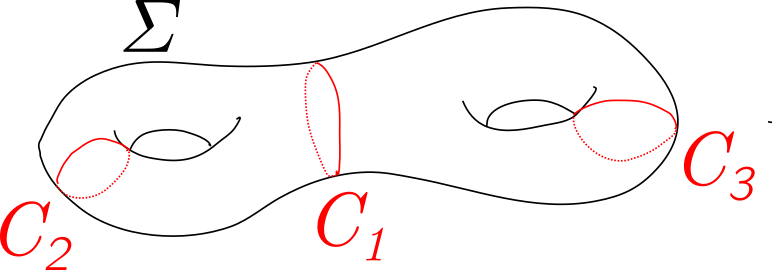
\includegraphics[width=0.5\linewidth]{genus2.png}\label{f:decompasym}}
		\subfloat[][The symmetric decomposition.]{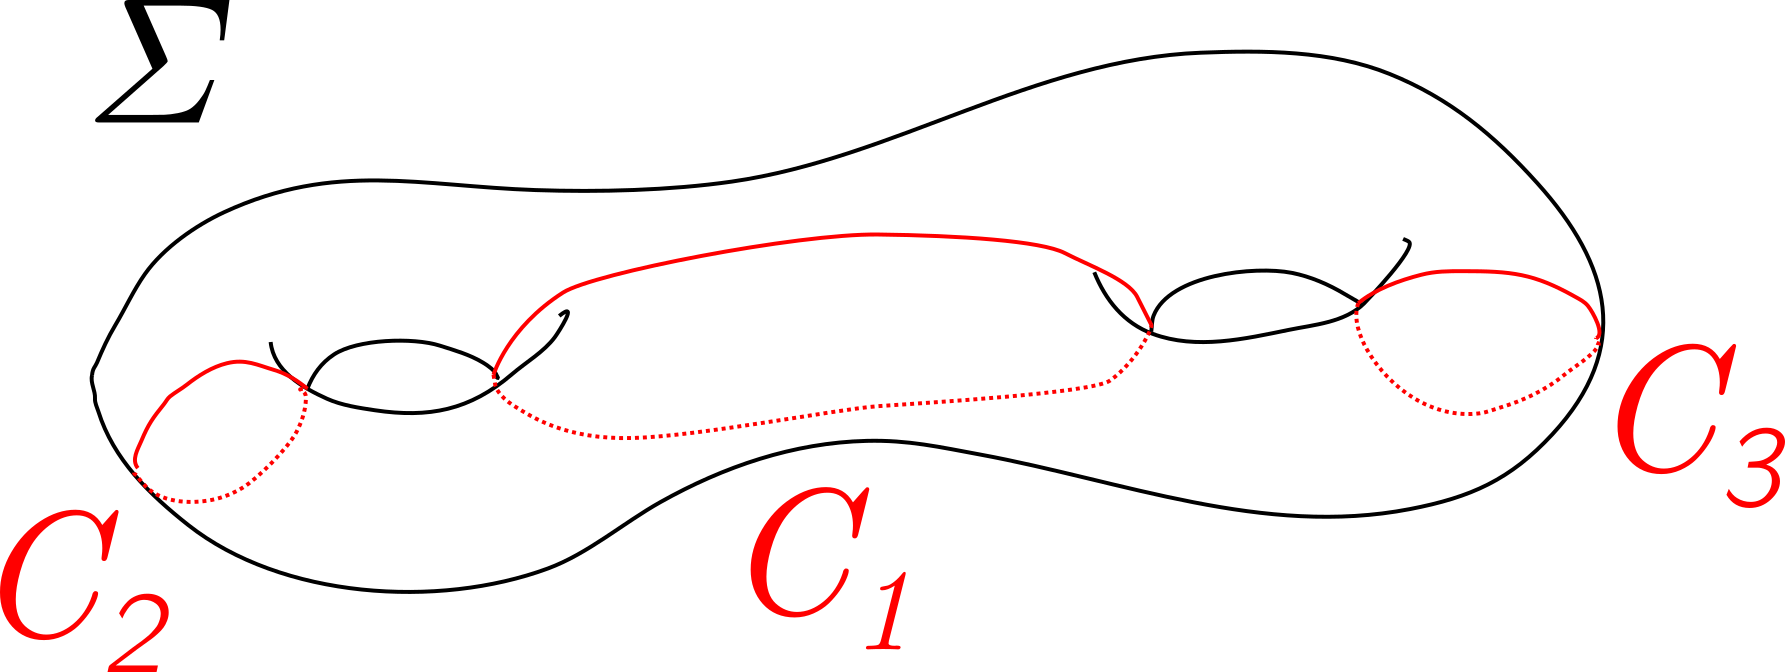
\includegraphics[width=0.5\linewidth]{g2sym.png}\label{f:decompsym}}
		\caption{The two possible trinion decompositions of a surface of genus $g=2$.}
	\end{figure}
	
	
	First consider the symmetric decomposition. Then the anti-diagonal action of $(\C^\ast)^3$ on $\PP^3\times \PP^3$ is given by
	\begin{align*}
		(\lambda, \mu,\nu)\cdot [x:y:z:w] &= [x:\lambda \mu y: \lambda \nu z: \mu\nu w]\\
		(\lambda, \mu,\nu)\cdot [x':y':z':w'] &= [x:\lambda^{-1} \mu^{-1} y: \lambda^{-1} \nu^{-1} z: \mu^{-1}\nu^{-1} w].
	\end{align*}
	Embedding $\PP^3\times \PP^3$ into $\PP^{15}$ (and defining the image as $X$), to compute the quotient we must find the graded ring of homogeneous invariant functions of Segre co-ordinates under the $(\C^\ast)^3$ action. Consider the polynomial $(x^\alpha y^\beta z^\gamma w^\delta x'^{\alpha'} y'^{\beta'} z'^{\gamma'} w'^{\delta'})$; the power of $\lambda,\mu$ and $\nu$ one gains from the action of $(\C^\ast)^3$ can be computed by the matrix-vector multiplication
	\begin{equation}
		\begin{bmatrix}
		p_\lambda \\
		p_\mu \\
		p_\nu \\
		\end{bmatrix} = \begin{bmatrix}
		1 & 1 & 0 & -1 & -1 & 0\\
		1 & 0 & 1 & -1 & 0 & -1\\
		0 & 1 & 1 & 0 & -1 & - 1\\
		\end{bmatrix}\begin{bmatrix}
		\beta \\
		\gamma \\
		\delta \\
		\beta' \\
		\gamma'\\
		\delta '\\
		\end{bmatrix}.
	\end{equation}
	Therefore, to find invariant polynomials, we can set $p_\lambda = p_\mu = p_\nu =0$ and row-reduce the matrix to find the powers of each co-ordinate which yield an invariant polynomial. Putting the matrix into row-reduced echelon form, we obtain $[\mathds{1}_{3}, -\mathds{1}_3]$ which means the only possible invariant polynomials are those with $\beta = \beta'$, $\gamma = \gamma'$ and $\delta = \delta'$. For the polynomials to be homogeneous, we need $\alpha+\beta+\gamma+\delta = \alpha'+\beta'+\gamma'+\delta'$, and therefore $\alpha = \alpha'$ as well. Hence, the degree-1 polynomials in the Segre co-ordinates are
	\begin{equation}
		xx', yy', zz' \text{ and } ww'.
	\end{equation}
	The ring of invariant functions is $\C[xx',yy',zz',ww']$, graded in the standard way, and the moduli space is given by the GIT quotient
	\begin{equation}
		\cP = (\PP_3 \times \PP_3)\sslash (\C^\ast)^3 = \text{Proj} \left(\C[xx',yy',zz',ww']\right) = \PP^3.
	\end{equation}
	Now, let us consider the asymmetric decomposition. In this case, the $(\C^\ast)^3$ action is
	\begin{align*}
	(\lambda, \mu,\nu)\cdot [x:y:z:w] &= [x:y: \lambda \mu z: \lambda\mu^{-1} w]\\
	(\lambda, \mu,\nu)\cdot [x':y':z':w'] &= [x: y: \lambda^{-1} \nu z: \lambda^{-1}\nu^{-1} w].
	\end{align*}
	The corresponding linear system for invariant polynomials is therefore
		\begin{equation}
	\begin{bmatrix}
	p_\lambda \\
	p_\mu \\
	p_\nu \\
	\end{bmatrix} = \begin{bmatrix}
	0 & 1 & 1 & 0 & -1 & -1\\
	0 & 1 & -1 & 0 & 0 & 0\\
	0 & 0 & 0 & 0 & 1 & -1\\
	\end{bmatrix}\begin{bmatrix}
	\beta \\
	\gamma \\
	\delta \\
	\beta' \\
	\gamma'\\
	\delta '\\
	\end{bmatrix}.
	\end{equation}
	Therefore, the $\alpha$s and $\beta$s are free variables, but $\gamma = \delta$ and $\gamma' = \delta'$. We also must have that $\gamma+\delta = \gamma'+\delta'$. The condition for homogeneity of degree gives one more constraint, that $d=\alpha+\beta+\gamma+\delta = \alpha + \beta + 2\gamma$. Therefore, the set of degree-1 invariant polynomials is
	\begin{equation}
		xx', yy', xy', yx'.
	\end{equation}
	However in this case, the degree-2 invariant polynomials are not all generated by products of the degree-1 invariants. We have the additional invariants
	\begin{equation}
		(ww')(zz'), (wz')(zw').
	\end{equation}
	The degree-2 invariants are the same polynomial, and the degree-1 invariants have one relation. The graded ring of invariant polynomials is $R=\C[a,b,c,d,e]/\langle ab-cd\rangle$, where $e$ has weight two. Taking the homogenous spectrum we obtain a variety inside the weighted projective space $\PP(1,1,1,1,2)$ defined by the ideal $\langle ab-cd\rangle$.
	
	For the symmetric gluing, we have $\OO(1)(\cP) = \text{span}\{xx',yy',zz',ww'\}$ which is dimension 4. Similarly, $\dim \OO(2)(\cP) = 4+\binom{4}{2} = 10$, from 4 squared functions and 6 cross-terms. For the asymmetric gluing, $\OO(1)(\cP) = \text{span}\{xx',yy',xy',yx'\}$ which is also dimension 4. Then these give 4 squared functions and 5 cross-terms, as $xx'yy' = xy'yx'$. The missing section is $ww'zz' = wz'zw'$, giving again $\dim\OO(2)(\cP) = 10$. We see that in each of these gluings, the number of sections of $\OO(n)$ agrees with the Verlinde formula of integer graph labellings that we computed in Section \ref{s:counting}.